\chapter{Metodología}
% Compactación de la energía será relevante mencionar en marco teórico
El diseño de este trabajo se basa en la implementación novedosa de los conceptos descritos anteriormente en el marco teórico. Como la mayoría de los esquemas de compresión, la propuesta aquí descrita implementa modificaciones sobre un desarrollo base que pretenden mejorar los resultados de compresión integrando nuevas metodologías para privilegiar la compactación de la energía de aquellos elementos más informativos de la señal.

\section{Esquema de compresión}
    Privilegiando la comprensión del lector, los siguientes diagramas muestran de forma general las etapas del esquema de compresión. El primero muestra el flujo de los datos geométricos y dónde precisamente en el esquema completo de compresión está ubicado el algoritmo propuesto. El segundo muestra el esquema de compresión propuesto con las etapas utilizadas para el presente trabajo, las cuales se ahondarán durante este capítulo.

    \begin{figure}
        \centering
        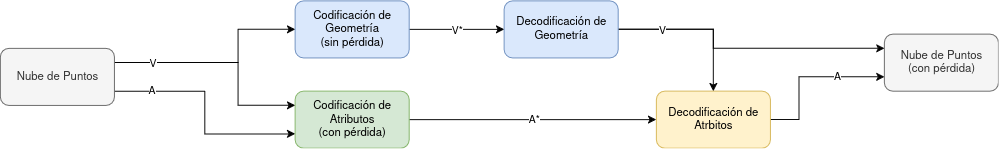
\includegraphics[width=1\textwidth]{img/metodología/Full-Scheme.png}
        \caption{Esquema completo de compresión}
        \label{fig:enter-label}
    \end{figure}

    En la figura anterior, se muestra la geometría de la nube de puntos conocida y sin pérdida tanto por el codificador como por el decodificador de atributos. Lo anterior es fundamental, pues permite a la implementación asumir la geometría como conocida y, por tanto, la utiliza sin agregar información adicional al flujo de bits. Entendiendo esto, la siguiente figura muestra el esquema de codificación propuesto para los atributos de color de la nube de puntos.

    \begin{figure}
        \centering
        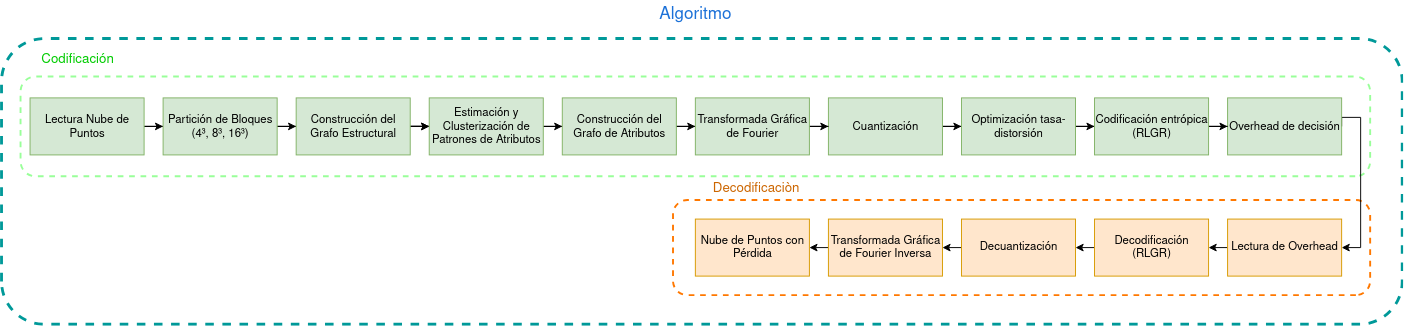
\includegraphics[width=1\textwidth]{img/metodología/PCADC_Algorithm_Hor.png}
        \caption{Esquema algoritmo compresión de atributos}
        \label{fig:enter-label}
    \end{figure}

\section{Datos Utilizados}
% - Describir el dataset utilizado (nombre, resolución, fuente, etc.)
    Lo primero a mencionar son las características de los datos utilizados para la evaluación de la metodología que se describirá a continuación, en tanto que esto condiciona el procesamiento en su posterioridad. \\

    Existen distintas formas de obtener datos de nubes de puntos, que limitan la resolución y caracterizan los datos en tanto su cantidad máxima de puntos y las referencias espaciales máximas que se pueden representar. En este trabajo se utilizaron dos bases de datos clásicas y ampliamente estudiadas en el campo de compresión de nubes de puntos.\\

    De forma general, ambas fuentes de datos contienen nubes de puntos descritas de la misma manera con metodologías de obtención distintas lo que implica ciertas diferencias de su contenido lo que condiciona el análisis posterior. Sin embargo la representación es la misma y consiste en un conjunto de puntos espacialmente ubicados según ejes cartesianos ($x$, $y$, $z$) restringidos por una grilla rectangular en 3D que sin pérdida de generalidad se asumen pertenecientes a un enmallado de números enteros.\cite{deon2017voxelized} Se dice de manera formal, que cada uno de estos puntos cartesianos se ubica en la grilla a través de un \textit{voxel}, que sería el equivalente a un pixel para un objeto tridimensional. En este contexto, se habla de que ambas fuentes de datos, poseen nubes de puntos voxelizadas cuya cantidad de puntos es no homogenea. Es importante destacar además que los \textit{voxeles} pueden estar tanto ocupados como desocupados, a diferencia de una imagen que posee información de color y señal en cada uno de sus píxeles, lo que justifica la búsqueda de estructuras no convencionales para la representación de la señal.\\
    
    \subsection{\textit{8i Voxelized Full Bodies}}
        Para este primer caso, principal caso de análisis por su complejidad y diversidad de fuentes, se trata de cuatro secuencias dinámicas de un sujeto en movimiento ocupando distintas vestimentas. Las secuencias están tipificadas como \textit{Long Dress}, \textit{Loot}, \textit{Red and Black} y \textit{Soldier} cada una capturada de treinta frames por segundo en un periodo de diez segundos, lo que considera aproximadamente 300 imágenes por secuencia.

        \begin{figure}[H]
            \centering
            \begin{subfigure}[b]{0.22\linewidth}
                \centering
                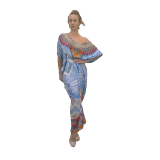
\includegraphics[width=\linewidth]{img/metodología/longdress_thumb.png}
                \caption{Longdress}
                \label{fig:longdress}
            \end{subfigure}
            \begin{subfigure}[b]{0.22\linewidth}
                \centering
                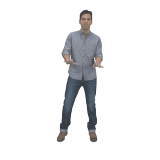
\includegraphics[width=\linewidth]{img/metodología/loot_thumb.png}
                \caption{Loot}
                \label{fig:loot}
            \end{subfigure}
            \begin{subfigure}[b]{0.22\linewidth}
                \centering
                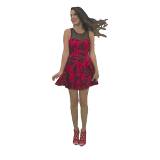
\includegraphics[width=\linewidth]{img/metodología/redandblack_thumb.png}
                \caption{Red and Black}
                \label{fig:redandblack}
            \end{subfigure}
            \begin{subfigure}[b]{0.22\linewidth}
                \centering
                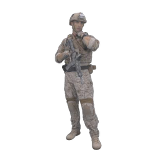
\includegraphics[width=\linewidth]{img/metodología/soldier_thumb.png}
                \caption{Soldier}
                \label{fig:soldier}
            \end{subfigure}
            \caption{Ejemplos Base de Datos - 8iVFB v2.}
            \label{fig:datasets}
        \end{figure}

        Estos datos fueron obtenidos a través de cuarenta y dos cámaras RGB configuradas en catorce agrupaciones donde cada uno de estas, actua logicamente como una cámara de cuatro canales incluyendo la reflectancia. Se ocupa la misma resolución espacial para cada una de las secuencias: un cubo de profundidad diez, es decir, una grilla de $2^{10} = 1024$ posiciones por orientación, entregando un total de $2^{10^{3}} \approx 1.07e9$ posibles posiciones. De todas maneras, para cada secuencia el cubo es escalado para ser el cubo delimitador más pequeño posible que contenga la secuencia. Es importante destacar que como típicamente la altura del sujeto es la dimensión más grande de la secuencia, la proporcionalidad en sistema internacional de los vóxeles estará dada por la siguiente expresión: 
        \begin{equation}
         \text{proporción} \frac{[m]}{[voxel]} \approx \frac{\text{altura}\;[m]}{1024 \; [voxels]}
        \end{equation}

        Para generar cierto tipo de intuición, para un sujeto de $1.8$ metros tendremos aproximadamente $1.75$ milímetros por voxel. Lo que implica que son objetos pensados para percibir a distancia.\\
        % - Justificar la elección del conjunto de datos
        Luego, la relevancia de este conjunto está principalmente en la diversidad de color, una mayor continuidad y la compresión en contexto de cuerpo completo.

    \subsection{\textit{Microsoft Voxelized Upper Bodies}}
        Este conjunto de datos a diferencia del anterior, consiste en imágenes de los troncos superiores de cinco sujetos catalogados como: \textit{Andres}, \textit{David}, \textit{Phil}, \textit{Ricardo} y \textit{Sara}. Cada uno de estos sujetos son capturados en siete y diez segundos completando dos secuencias. Las secuencias más cortas están capturadas con profundidad nueve, es decir, una grilla de $2^{9^{3}}$, mientras las más largas con una profundidad de diez.\\
        La obtención de estos datos se hizo mediante cuatro cámaras RGBD a treinta cuadros por segundo entregando un total de 210 y 300 imágenes para cada versión respectiva. Como es razonable, la profundidad cambia la resolución de la nube de puntos donde aproximadamente los voxeles de profundidad nueve corresponden a $1.5\;[mm]$ cúbicos mientras que las de profundidad diez corresponden a $0.75\;[mm]$ cúbicos. \cite{loop2016microsoft} 

        \begin{figure}[H]
            \centering
            \begin{subfigure}[b]{0.19\linewidth}
                \centering
                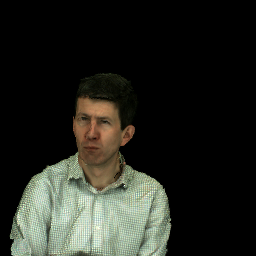
\includegraphics[width=\linewidth]{img/metodología/andrew_thumb.png}
                \caption{Andrew}
                \label{fig:andrew}
            \end{subfigure}
            \begin{subfigure}[b]{0.19\linewidth}
                \centering
                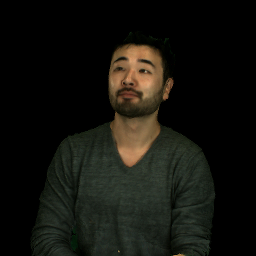
\includegraphics[width=\linewidth]{img/metodología/david_thumb.png}
                \caption{David}
                \label{fig:david}
            \end{subfigure}
            \begin{subfigure}[b]{0.19\linewidth}
                \centering
                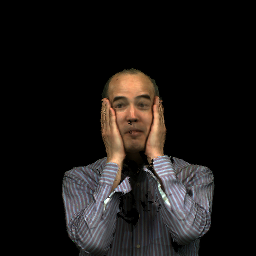
\includegraphics[width=\linewidth]{img/metodología/phil_thumb.png}
                \caption{Phil}
                \label{fig:phil}
            \end{subfigure}
            \begin{subfigure}[b]{0.19\linewidth}
                \centering
                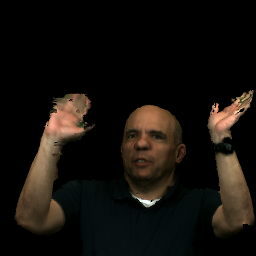
\includegraphics[width=\linewidth]{img/metodología/ricardo_thumb.png}
                \caption{Ricardo}
                \label{fig:ricardo}
            \end{subfigure}
            \begin{subfigure}[b]{0.19\linewidth}
                \centering
                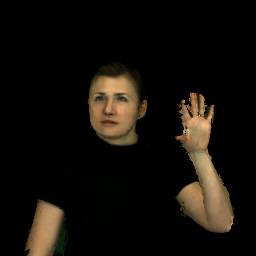
\includegraphics[width=\linewidth]{img/metodología/sarah_thumb.png}
                \caption{Sarah}
                \label{fig:sarah}
            \end{subfigure}
            \caption{Ejemplos Base de Datos - MVUB.}
            \label{fig:seq_immersive}
        \end{figure}
        % - Justificar la elección del conjunto de datos
        En este caso, este conjunto se caracteriza entonces por una resolución más fina y es relevante para observar el desempeño del algoritmo a corta distancia. Para análisis cualitativos será fundamental observar como se diferencia el desempeño del método entre este conjunto de datos y el anterior. 

    Finalmente es importante mencionar que ambas bases de datos presentan las nubes de puntos indexadas según el orden de Morton explicado en el marco teórico. Este orden privilegia la cercanía indexada de aquellos puntos que poseen mayor cercanía representándolos como una lista unidimensional.
    
\section{Partición de la Nube de Puntos}
    % - Explicar el proceso de división en bloques (por ejemplo, tamaños 4³, 8³, 16³)
    % - Justificar la necesidad de particionar
    % - Relación con la adaptabilidad local del método
    De la misma forma que los métodos clásicos implementan el paradigma de divide y vencerás para los problemas computacionales, la compresión de nubes de puntos tiene como primer paso la división por bloques. Lo que sería tradicionalmente una división de una imagen en ventanas de cierta cantidad de pixeles, aquí se divide el espacio en cubos de cierta cantidad de vóxeles.\\

    En este contexto, lo primero es mencionar que los tamaños de bloques deben ser potencias de dos, ya que como se mencionó en la sección anterior, la profundidad de resolución se corresponde con potencias binarias. Por lo tanto la siguiente expresión limita la posibilidad de tamaños de bloques según lo siguiente:

    \begin{equation}
        b = 2^k, \quad k \in \mathcal{N}
    \end{equation}

    Luego, se operan las coordenadas según dicho tamaño de bloque con el objetivo de determinar como los puntos se ubican dentro de estas nuevas celdas tridimensionales. Matemáticamente se hace una cuantización escalar la cuál nos entrega la frontera más cercana para los bloques del tamaño elegido. Sea $v_i$ la posición del punto para el índice $i$.

     \begin{equation}
         v^{block}_i = \left\lfloor \frac{v_i}{b} \right\rfloor \cdot b
     \end{equation}

     De esta manera, se mapea cada punto al origen del bloque cúbico al que pertenece. Por ejemplo, si $b=8$, un punto $(13,7,19)$ se mapea a $(0, 8,16)$ indicando la pertenencia al bloque de dicho origen. Luego, es fácil observar que si a estos puntos cuantizados les calculamos sus diferencias podemos encontrar aquellos donde existen cambios de bloques, identificando precisamente la pertenencia de cada punto. Matemáticamente describimos la siguiente métrica:

     \begin{equation}
         \Delta _i = || v^{block}_{i+1} - v^{block}_i ||_1
     \end{equation}

     Donde, encontraremos los puntos que pertenecen a cierto bloque siempre y cuando $\Delta_i = 0$ para las distintas comparaciones entre puntos. Esto nos entregará un conjunto de índices, que gracias al orden de Morton, son secuenciales y por tanto se representan por su índice inicial y final.\\

     A modo de ejemplo, la siguiente figura muestra el primer bloque de la secuencia \textit{Long Dress} para un tamaño de bloque de dieciséis.
     \begin{figure}
         \centering
         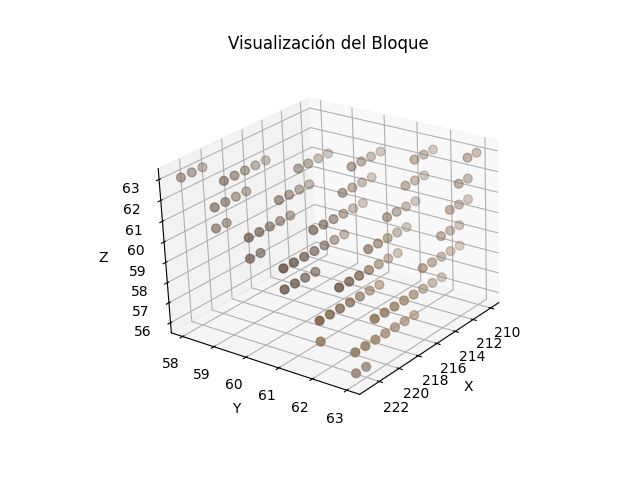
\includegraphics[width=0.8\linewidth]{img/metodología/Bloque_Ejemplo.png}
         \caption{Ejemplo de Bloque ($b=16$)}
         \label{fig:enter-label}
     \end{figure}les.\\

    En este contexto, lo primero es mencionar que los tamaños de bloques deben ser potencias de dos, ya que como se mencionó en la sección anterior, la profundidad de resolución se corresponde con potencias binarias. Por lo tanto la siguiente expresión limita la posibilidad de tamaños de bloques según lo siguiente:

    \begin{equation}
        b = 2^k, \quad k \in \mathcal{N}
    \end{equation}

    Luego, se operan las coordenadas según dicho tamaño de bloque con el objetivo de determinar como los puntos se ubican dentro de estas nuevas celdas tridimensionales. Matemáticamente se hace una cuantización escalar la cuál nos entrega la frontera más cercana para los bloques del tamaño elegido. Sea $v_i$ la posición del punto para el índice $i$.

     \begin{equation}
         v^{block}_i = \left\lfloor \frac{v_i}{b} \right\rfloor \cdot b
     \end{equation}

     De esta manera, se mapea cada punto al origen del bloque cúbico al que pertenece. Por ejemplo, si $b=8$, un punto $(13,7,19)$ se mapea a $(0, 8,16)$ indicando la pertenencia al bloque de dicho origen. Luego, es fácil observar que si a estos puntos cuantizados les calculamos sus diferencias podemos encontrar aquellos donde existen cambios de bloques, identificando precisamente la pertenencia de cada punto. Matemáticamente describimos la siguiente métrica:

     \begin{equation}
         \Delta _i = || v^{block}_{i+1} - v^{block}_i ||_1
     \end{equation}

     Donde, encontraremos los puntos que pertenecen a cierto bloque siempre y cuando $\Delta_i = 0$ para las distintas comparaciones entre puntos. Esto nos entregará un conjunto de índices, que gracias al orden de Morton, son secuenciales y por tanto se representan por su índice inicial y final.\\

     A modo de ejemplo, la siguiente figura muestra el primer bloque de la secuencia \textit{Long Dress} para un tamaño de bloque de dieciséis.
     \begin{figure}
         \centering
         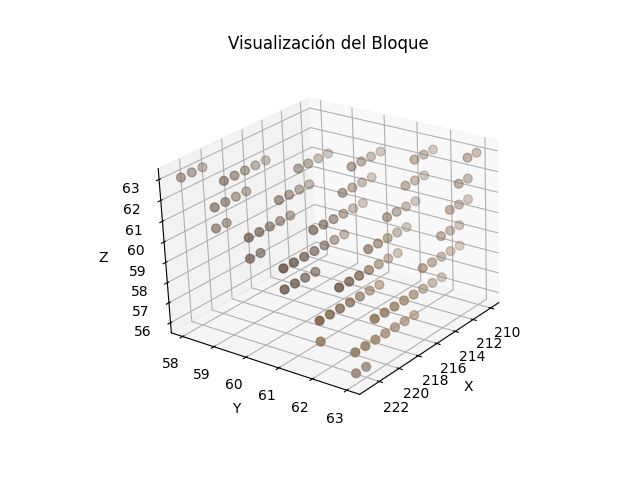
\includegraphics[width=0.8\linewidth]{img/metodología/Bloque_Ejemplo.png}
         \caption{Ejemplo de Bloque ($b=16$)}
         \label{fig:enter-label}
     \end{figure}
    
    % DAR UN EJEMPLO??? + Visual
\section{Construcción del Grafo Estructural}
% - Explicar cómo se conecta cada punto con sus vecinos
% - Tipo de conectividad usada (k-NN, radio, etc.)
% - Qué representa el grafo: estructura geométrica de la nube
    La implementación del método se basa fuertemente en la interacción de las muestras de forma local respecto a su vecindad. Pero ninguno de estos conceptos hace sentido sin una estructura subyacente a la cuál se le pueda entregar esta interpretación. Por otro lado, como se mencionó en la primera sección de este capítulo, el desarrollo está sustentado bajo la hipótesis de que tanto el codificador como el decodificador están en pleno conocimiento de la geometría de la nube. Con esto en mente entonces, es relevante para el método propuesto aprovechar al máximo la información espacial para la compresión para evitar la necesidad de información adicional.\\

    Considerando lo anterior, el primer paso es construir el grafo estructural por bloque, esto está definido de la misma manera que se mencionó en la sección \ref{sec: pcac_geometric}. Esta será la estructura adyacente, donde lo importante a notar que la relación de los nodos están dados por la diagonal cúbica unitaria y los pesos serán inversamente proporcionales a dicha distancia.\\

    Finalmente, es importante notar que cada nodo puede tener una multiplicidad de vecinos no homogénea, lo que diferencia esta estructura a lo que sería el paradigma clásico de imágenes. Lo anterior implica que este grafo puede tomar muchas formas y cada nodo posee una cantidad distinta de vecinos, para ilustrar esto se presenta la siguiente figura:

    \begin{figure}
        \centering
        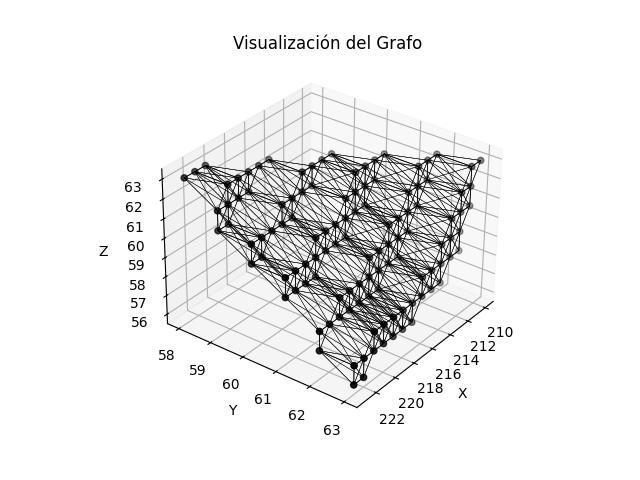
\includegraphics[width=0.85\linewidth]{img/metodología/Grafo_Ejemplo.png}
        \caption{Ejemplo de Grafo ($b=16$)}
        \label{fig:enter-label}
    \end{figure}
    % SERÁ NECESARIO DECIR ALGO MÁS??? O desarrollar mejor el estado del arte


\section{Análisis de Patrones de Atributos}
    % AUN EN DESARROLLO
    Hasta ahora, toda la metodología ha trabajado con los datos espaciales de la nube de puntos. Sin embargo, el objetivo radica en la compresión de los atributos, lo que podría llamarse los valores de la señal. Atacando lo anterior y usando la lógica heredada de métodos clásicos de codificación basado en transformadas (\ref{sec:transform_based_coding}).\\

    La presente implementación se enfoca en atributos de color RGB, por tanto, el primer paso intuitivo es hacer la transformación que cualitativamente es más informativa descrita por el algoritmo JPEG. En otras palabras, se transforma el espacio de color RGB al espacio YUV sin pérdida de información. Luego, como se mencionó en la sección \ref{subsubsec: jpeg} lo más relevante será privilegiar la información en el canal de luminancia al ser esta para la cual el ojo humano posee mayor resolución.\\

    El presente método de compresión tiene como objetivo declarado ocupar la información de los atributos para establecer un método dependiente de compresión adaptando la estructura del grafo. No obstante, es impracticable la transmisión de los atributos para su utilización tanto así como las decisiones crudas derivadas de ello. Lo anterior, motiva el dilema de transmitir una representación óptima de la información necesaria o de las decisiones tomadas. Optando por lo primero, el objetivo de esta sección es mostrar una estrategia para transmitir representaciones aproximadas de la información de los atributos con un conjunto de bases limitadas.\\

    Por supuesto, para poder lograr esto se hace indispensable la normalización de los bloques para que las representaciones sean atribuibles y clusterizables entre todas. Por tanto, el primer paso es la normalización posicional y rotacional del bloque.

    \subsection{Normalización Espacial}
        Lo primero es centrar los puntos del bloque para elaborar referencias de bloques uniformes. Esta operación es simple y consiste en remover la media por componente al conjunto de puntos del bloque:

        \begin{equation}
            V_i^{c} = V_{i} - \bar{V_i}
        \end{equation}

        Posterior a esto, es relevante orientar todos los bloques en los ejes virtuales donde su variación es máxima. El objetivo de aquellos es que aquellos bloques que representen distribuciones espaciales similares tengan una expresión similar. Para aquellos lo primero es definir la matriz de covarianza del bloque que expresa matemáticamente la variación de cada componente sobre si mismo y entre ellos:

        \begin{equation}
            \mathbf{\Sigma} =
                \begin{bmatrix}
                \mathrm{Var}[x] & \mathrm{Cov}[x,y] & \mathrm{Cov}[x,z] \\
                \mathrm{Cov}[y,x] & \mathrm{Var}[y] & \mathrm{Cov}[y,z] \\
                \mathrm{Cov}[z,x] & \mathrm{Cov}[z,y] & \mathrm{Var}[z]
                \end{bmatrix}
        \end{equation}

        A partir de aquello, podemos encontrar las bases ortogonales que representan la mayor variación del bloque. Para aquello hacemos la descomposición en vectores propios:

        \begin{equation}
            \mathbf{\Sigma} = \mathbf{Q} \mathbf{\Lambda} \mathbf{Q}^\top
        \end{equation}

        Si bien estos vectores propios poseen la rotación en el sentido específicado. Existe la posibilidad de que la rotación genere un efecto espejo, perdiendo la uniformidad de la transformación para todos los bloques. En este sentido, forzamos que el tercer vector propio cumpla con la regla de la mano derecha, o más formalmente que la orientación de la base ortonormal sea positiva.

        \begin{equation}
            \mathbf{q}_3 = \mathbf{q}_1 \times \mathbf{q}_2
        \end{equation}
        
        Con estas bases canónicas rotamos el bloque en las direcciones especificadas normalizando su orientación.
        \begin{equation}
            V^{r}_i = V^{c}_i \mathcal{}{Q}
        \end{equation}

        En el ejemplo presentado en las secciones anteriores, esto se vería de la siguiente forma:

        \begin{figure}
            \centering
            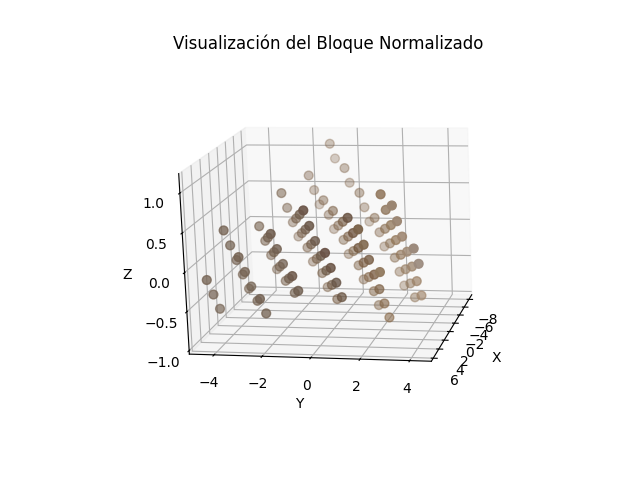
\includegraphics[width=0.85\textwidth]{img/metodología/Norm_Ejemplo.png}
            \caption{Ejemplo de Normalización (b=16)}
            \label{fig:enter-label}
        \end{figure}

        
    \subsection{Aproximación lineal}
        Una vez que cada bloque es comparable entre sí por el paso anterior, el objetivo es encontrar una representación del canal objetivo (luminancia) que pueda aproximar las dinámicas espaciales. Para aquello, se utiliza una aproximación lineal, que mapea las posiciones de los vóxeles con una aproximación de color de la forma:
        
        \begin{equation}
            \hat{y} = f(x,y,z) = \beta^\top \Phi = \beta_0 + \beta_1x + \beta_2y + \beta_3z
        \end{equation}
        
        Encontrar esta aproximación se hace a través de una regresión polinomial que minimice el error cuadrático respecto al canal original. Sea $\Phi \in \mathbb{R}^{N \times M}$ la matriz de características que contiene los monomios evaluados en cada posición $(x_i, y_i, z_i)$, y sea $Y \in \mathbb{R}^{N}$ el vector de valores reales del canal de luminancia. Los coeficientes $\beta \in \mathbb{R}^M$ se encuentran resolviendo el siguiente problema de mínimos cuadrados:
        
        \begin{equation}
            \beta^* = \arg\min_{\beta} \| Y - \Phi \beta \|_2^2
        \end{equation}
        
        La solución cerrada de este problema está dada por:
        
        \begin{equation}
            \beta^* = (\Phi^\top \Phi)^{-1} \Phi^\top Y
        \end{equation}
        
        Donde $\Phi$ incluye un primer término constante (bias) y columnas para cada monomio involucrado según el grado polinomial. En el caso lineal, los términos son: $[1, x, y, z]$.
        
        

        
    \subsection{Clusterización}
        % Aun en desarrollo
        Finalmente, se tendrá un conjunto de coeficientes para cada bloque que considera una constante y tres valores que ponderan las posiciones espaciales \(x\), \(y\) y \(z\). Como la metodología propuesta se enfoca únicamente en la dinámica de los atributos a través de las posiciones relativas, el término constante \(\beta_0\) no es relevante para este análisis y se omite. De este modo, cada bloque \(i\) está representado por un vector de coeficientes:
        
        \[
        \tilde{\beta}_i^\top = 
        \begin{bmatrix}
        \beta_1 & \beta_2 & \beta_3
        \end{bmatrix}
        \in \mathbb{R}^{1 \times 3}
        \]
        
        y el conjunto completo de bloques se organiza en una matriz:
        
        \begin{equation}
            \tilde{\boldsymbol{\beta}} =
            \begin{bmatrix}
                \tilde{\beta}_1^\top \\
                \tilde{\beta}_2^\top \\
                \vdots \\
                \tilde{\beta}_N^\top
            \end{bmatrix}
            =
            \begin{bmatrix}
                \beta_1^{(1)} & \beta_2^{(1)} & \beta_3^{(1)} \\
                \beta_1^{(2)} & \beta_2^{(2)} & \beta_3^{(2)} \\
                \vdots & \vdots & \vdots \\
                \beta_1^{(N)} & \beta_2^{(N)} & \beta_3^{(N)}
            \end{bmatrix}
            \in \mathbb{R}^{N \times 3}
        \end{equation}
        
        
        donde cada fila corresponde a los coeficientes \((\beta_1, \beta_2, \beta_3)\) asociados a un bloque, en coherencia con la expresión general \(\hat{y} = \beta^\top \Phi\). Sobre este conjunto se quiere buscar el mínimo subconjunto que puede expresar las dinámicas generales de los bloques de la nube de puntos. Para ello, se implementa clusterización sobre el conjunto $\tilde{\boldsymbol{\beta}}$ encontrando el número de clusters que minimice la siguiente función:

        \begin{equation}
            J(\tilde{\boldsymbol{\beta}}, \mathbf{c}, \ell) = -\frac{1}{K} \sum_{k=1}^{K} \frac{1}{|C_k|} \sum_{\tilde{\beta}_i \in C_k} \|\tilde{\beta}_i - \mathbf{c}_k\|_2 + \lambda K
        \end{equation}
        Donde la función de costo $J$ balanceea dos objetivos complementarios:

        \begin{itemize}
            \item \textbf{Minimización de distancia intra-cluster (término negativo)}: El primer término, busca minimizar la distancia promedio entre los vectores de coeficientes y sus respectivos centroides $c_k$. Esto fomenta la formación de clusters compactos donde los bloques con dinámicas similares se agrupen.

            \item \textbf{Penalización por complejidad (término positivo)}: El término $\lambda K$ penaliza un número excesivo de clusters, actuando como regularizador para evitar la sobreparametrización del modelo. Un valor mayor de $\lambda$ favorece soluciones con menos clusters.
        \end{itemize}
        
        El objetivo es encontrar el valor óptimo de $K$ que minimice $J$, identificando así el número de patrones dinámicos fundamentales presentes en el conjunto de bloques. \\

        De la minimización de dicha función se encontrarán centroides $c_1,...,c_K$ los cuales describen las dinámicas de luminancia características de la señal. Para cada bloque $i$, se tomará la decisión de aproximación según el centroide que minimice el error de representación.
        
    % - Describir el modelo de estimación del atributo (p.ej., regresión lineal por bloque)
    % - Cómo se extraen características o dinámicas del atributo
    % - Método de clusterización usado para agrupar dinámicas similares
    % - Justificación para usar clusters como guía para bases transformadas

\section{Construcción del Grafo de Atributos}
    La modificación del grafo estructural es parte fundamental de este trabajo en tanto es la principal contribución al trabajo realizado por otros autores. Considerando lo mencionado en la sección de procesamiento de señales representadas por grafos \ref{sec: gsp}, la construcción del grafo modifica su representación en el espacio transformado, es en tanto, principal poder generar aprovechar la información de la señal con el propósito alcanzar bases más representativas.\\

    Incluir esta información en el caso de estudio, se basa en la idea presentada en la sección \ref{sec: lst_ice} de que las bases transformadas representadas por el grafo se ven afectadas localmente por el posicionamiento de \textit{self-loops}, es decir conexiones cíclicas de un nodo hacia si mismo. En este sentido, se implementan las siguientes estructuras matemáticas para la identificación estratégicas de dinámicas decrecientes de color por sobre la estructura declarada del grafo estructural.

    \subsection{Matriz de dinámica de atributos}
        Con el propósito de visualizar la dinámica del atributo entre vecinos. La matriz de atributos se define como:
        \begin{equation}
            M_{ij} = \frac{W_{ij} \cdot (y_i - y_j)}{255}
        \end{equation}

        Es importante notar que el peso asociado será no nulo solo si los nodos $v_i,v_j$ están conectados. De manera más formal:
        
        \begin{equation}
            W_{ij} \neq 0, \quad (i,j) \in \mathcal{E}
        \end{equation}

        Además la dinámica del color está ponderada por el peso, lo que es una proporcionalidad de la distancia entre dichos vecinos.
            
    \subsection{Vector de nodos sumideros}
        Lo siguiente es buscar para cada nodo $i$ el vecino $j$ donde el color decrece de manera más significativa. De otra manera, esto es una manera local de observar la dinámica del color.
        \begin{equation}
            S_j = \left| \left\{ i \mid j = \arg\min_{k} M_{ik}, \; W_{ik} > 0 \right\} \right|
        \end{equation}

        Esto entregará un conteo de cuantos vecinos decrecen en la dirección del nodo. Ahora, con el propósito de poder definir umbrales universales y relevar aquellos sumideros que eventualmente afectaran de manera más representativa a sus vecinos, se normaliza de la siguiente manera:

        \begin{equation}
            S_i \leftarrow \frac{S_i - \min(\mathbf{S})}{\max(\mathbf{S}) - \min(\mathbf{S})}
        \end{equation}
        
    \subsection{Selección de \textit{self-loops}}
        Finalmente la selección de los nodos estratégicos se realiza a través de un umbral estático por sobre todos los bloques evaluado en el vector de sumidero. El objetivo será privilegiar la implementación de self-loops en aquellos puntos que presentan una influencia mayor en el decaimiento del atributo. Para ello, se utiliza un umbral $\tau \in [0,1]$ que determina la relevancia suficiente para ser incluido. 

        \begin{equation}
            \mathcal{S} = \left\{ i \in \{1,\dots,N\} \mid S_i \geq \tau \right\}
        \end{equation}

        Sobre esta última lista, se agregan conexiones representadas por la matriz de adyacencia con un valor fijo $w_{sl}$ que se ven de la siguiente manera:

        \begin{equation}
            W_{ii} \leftarrow w_{\text{sl}}, \quad \forall i \in \mathcal{S}
        \end{equation}
% - Describir cómo se modifica el grafo estructural para incluir la señal
% - Introducción de self-loops u otros ajustes
% - Intuición detrás de adaptar la estructura según la señal

\section{Transformada Gráfica de Fourier}\label{sec: method_gft}

    Alcanzado este punto, existen un conjunto de grafos posibles los cuales entregarán distintas transformadas. Primero, tenemos el grafo de información estructural el cual solo tiene la construcción original. Esta transformada tiene la característica de tener una primera base plana.
    
    \subsection{Caso Base: Grafo sin Self-loops}
    
    Para el grafo estructural construido según la metodología de voxelización descrita anteriormente, la primera base eigenvector del Laplaciano $L = D - A$ corresponde al eigenvalor $\lambda_1 = 0$ y satisface:
    
    $$L\phi_1 = 0 \Rightarrow (D - A)\phi_1 = 0$$
    
    Debido a la estructura regular del grafo voxelizado y la conectividad basada en distancias discretas con pesos $w_1 = 1$, $w_2 = \frac{1}{\sqrt{2}}$, $w_3 = \frac{1}{\sqrt{3}}$, la primera base toma la forma aproximadamente plana:
    
    $$\phi_1 \approx \frac{1}{\sqrt{N}} \mathbf{1}_N = \frac{1}{\sqrt{N}} \begin{bmatrix} 1 \\ 1 \\ \vdots \\ 1 \end{bmatrix}$$
    
    Esta aproximación es válida debido a que la estructura voxelizada crea un patrón de conectividad localmente homogéneo, donde el operador Laplaciano actúa como un filtro de suavizado que fuerza la uniformidad en el primer eigenvector.
    
    Ocupando la notación presentada en \ref{subsec: gft}, decimos que $\phi_1$ representa una base constante que representa el promedio de las muestras. Dicha base plana funciona luego en los coeficientes transformados como una especie de constante en la representación lineal de la señal:
    
    $$x = \sum_{i=1}^{N} \hat{x}_i \phi_i = \hat{x}_1 \phi_1 + \sum_{i=2}^{N} \hat{x}_i \phi_i$$
    
    donde $\hat{x}_1 = \phi_1^T x \approx \frac{1}{\sqrt{N}} \sum_{j=1}^{N} x_j$ representa la componente de baja frecuencia (\textit{DC}) o promedio de la señal.
    
    \subsection{Caso Modificado: Grafo con Self-loops}
    
    A manera de contraste, la segunda implementación cambia la estructura de la matriz de adyacencia al añadir pesos a la diagonal (debido al efecto de los \textit{self-loops}). El Laplaciano generalizado toma la forma:
    
    $$L_g = D - A + C$$
    
    donde $C$ incluye los pesos de self-loops en la diagonal: ${c}_{ii} =  w^i_{sl}$.
    
    El efecto de lo anterior se visualiza en todas las bases, sin embargo, el principal efecto radica en la primera base la cual ahora representará un promedio ponderado inversamente. La nueva primera base satisface:
    
    $$L_g\tilde{\phi}_1 = \tilde{\lambda}_1 \tilde{\phi}_1$$
    
    donde $\tilde{\lambda}_1 > 0$ (ya no es cero debido a los self-loops).
    
    La primera base modificada toma la forma:
    
    $$\tilde{\phi}_1 = \frac{1}{\sqrt{\sum_{j=1}^{N} (d_j + w^j_{sl})^{-2}}} \begin{bmatrix} (d_1 + w^1_{sl})^{-1} \\ (d_2 + w^2_{sl})^{-1} \\ \vdots \\ (d_N + w^N_{sl})^{-1} \end{bmatrix}$$
    
    Esta expresión muestra cómo los nodos con self-loops (mayor $w^j_{sl}$) obtienen menor magnitud en la primera base, otorgando menor peso a esos datos en el promedio ponderado.
    
    \subsection{Comportamiento Dinámico}
    
    Lo anterior le entregará dinámica a la base observando el siguiente comportamiento para el grafo unitario:
    
    \begin{itemize}
       \item \textbf{Sin self-loops}: $\phi_1$ es constante, todos los nodos contribuyen igualmente al promedio
       \item \textbf{Con self-loops}: $\tilde{\phi}_1$ es variable, los nodos con self-loops contribuyen menos al promedio ponderado
    \end{itemize}
    
    El coeficiente transformado correspondiente será:
    
    \begin{equation}
        \hat{\tilde{x}}_1 = \tilde{\phi}_1^T x = \frac{\sum_{j=1}^{N} (d_j + w^j_{sl})^{-1} x_j}{\sqrt{\sum_{j=1}^{N} (d_j + w^j_{sl})^{-2}}}
    \end{equation}
    
    Este comportamiento permite una representación más adaptativa donde la importancia de cada nodo en la componente de "promedio" puede ser controlada mediante los pesos de self-loops $w^j_{sl}$. 
% - Detallar la GFT usada
% - Cómo se obtienen y seleccionan las bases
% - Rol del clustering en la selección de la base para cada bloque

\section{Cuantización}

    Hasta ahora, ninguno de los procesos incluye pérdida de información, ya que todos los procesos son invertibles, sin embargo, para el proceso de compresión es importante disminuir la calidad de la información de forma estratégica para disminuir la codificación de datos poco perceptibles.
    
    \subsection{Cuantización Escalar Uniforme}
    
    Es por lo anterior, que el paso de cuantización implicará pérdidas con enfoque especial en aquellos coeficientes transformados de menor magnitud, es decir, que aportan menos a la señal. La magnitud relativa de cada coeficiente está dada por:
    
    $$\text{Contribución}_i = \frac{|\hat{x}_i|^2}{\sum_{j=1}^{N} |\hat{x}_j|^2}$$
    
    donde coeficientes con menor contribución son candidatos prioritarios para cuantización agresiva.
    
    Con dicho objetivo, se implementa una cuantización escalar uniforme con una lista de valores fijos ($Q_{set}$) para todos los experimentos. Sea $\hat{x}$ los coeficientes transformados para cierto bloque:
    
    $$q(\hat{x}) = \left\lfloor \frac{1}{q_{step}}\hat{x} \right\rceil,\quad q_{step} \in Q_{set}$$
    
    El proceso de reconstrucción está dado por:
    
    $$\hat{x}_{rec} = q_{step} \cdot q(\hat{x})$$
    
    introduciendo un error de cuantización acotado: $|\hat{x} - \hat{x}_{rec}| \leq \frac{q_{step}}{2}$.
    
    Donde $Q_{set}$ dependerá de las necesidades del experimento, pero principalmente restringe el rango de valores en los cuales se encontrará eventualmente las métricas de tamaño y calidad de la nube de puntos. Generalmente $Q_{step} \subset \{1,2,4,8,16,24,28,32,40,48,56,64\}$ un subconjunto de valores enteros múltiplos de $2$.
    
    \subsection{Efecto Espectral de la Cuantización}
    
    El efecto esperado de esta operación es la eliminación de aquellas bases que reflejan ruido o dinámicas locales demasiado específicas y con baja influencia global en la señal. Dicha influencia está representada por los coeficientes transformados que además representan bases ordenadas en función de los valores propios $\lambda_1 \leq \lambda_2 \leq \ldots \leq \lambda_N$, es decir, en bajas frecuencias de influencia global a altas frecuencias de influencia local.
    
    La probabilidad de que un coeficiente se cuantice a cero está dada por su pertenencia al conjunto $\left(-\frac{1}{2},\frac{1}{2}\right)$:
    
    $$P(\hat{x}_i \to 0) = P\left(|\hat{x}_i| < \frac{q_{step}}{2}\right)$$
    
    donde típicamente $P(\hat{x}_i \to 0)$ aumenta para coeficientes de alta frecuencia (grandes $\lambda_i$) debido a su menor magnitud esperada.
    
    \subsection{Distribución Post-Cuantización}
    
    Considerando lo anterior, la distribución esperada de los coeficientes transformados cuantizados, a mayor paso de cuantización concentrará mayor cantidad de valores nulos a través de la aproximación de valores decimales. La fracción de coeficientes cero puede aproximarse como:
    
    $$f_{zero} \approx \sum_{i=1}^{N} P(\hat{x}_i \to 0) \cdot \frac{1}{N}$$
    
    Esta distribución es idónea para el codificador por entropía utilizado que se detallará más adelante ya que:
    
    \begin{enumerate}
        \item Una concentración continua de valores en cero (alta $f_{zero}$) privilegia la codificación por longitud
        \item Una distribución predecible pre-ordenada por magnitud de valores propios privilegia el proceso de la parte entrópica del método \textit{Golomb-rice}
    \end{enumerate}

% - Tipo de cuantización empleada (uniforme, escalonada, etc.)
% - Cómo se adapta la cuantización a cada bloque o cluster
% - Relación con la tasa-distorsión

\section{Optimización Tasa-Distorsión}
    Una vez se tiene la información con pérdida, debemos considerar que se tienen un conjunto de transformadas y aproximaciones de color sobre las cuáles se debe decidir de manera óptima. Como se mencionó en la sección \ref{sec: rdt}, para los métodos de compresión esta optimización se debe evaluar sobre métricas de distorsión y restricciones de tamaño haciendo una optimización de lagrange según la ecuación \ref{eq: rdo_lagrange}.\\

   En este sentido, la implementación presenta un conjunto de desafíos a resolver para poder hacer uso práctido de la expresión anterior. Ya que considera elementos que no son determinables a priori y por tanto es necesario encontrar expresiones aproximadas de sus valores.

    \subsection{Métricas de distorsión}
    
    En primer lugar, al referirse a métricas de distorsión este trabajo prioriza la calidad del color por tanto uno esperaría trabajar sobre la diferencia de la información original y la recuperada posterior a la cuantización y codificación. Sin embargo, el objetivo de la optimización es poder tomar la decisión antes de este proceso, es por ello que entendiendo que el proceso descrito en la sección \ref{sec: method_gft} es invertible, es válido trabajar sobre los coeficientes transformados y su cuantización para evaluar la distorsión.
    
    \subsubsection{Distorsión Base}
    
    Es por aquello, que definimos la distorsión aportada a la ecuación de optimización de la forma:
    
    \begin{equation}
        d_{ij} = ||\hat{x} - q^{-1}(q(\hat{x}))||_2 = ||\hat{x} - \left\lfloor \frac{\hat{x}}{q_{step}} \right\rceil \cdot q_{step}||_2 
    \end{equation}
    
    donde $q^{-1}(q(\hat{x})) = \left\lfloor \frac{\hat{x}}{q_{step}} \right\rceil \cdot q_{step}$ representa el proceso de cuantización seguido de reconstrucción. Esta será la configuración base para los experimentos realizados, donde esta no considera las diferencias de relevancia de los canales.
    
    \subsubsection{Ponderación por Componentes de Color}
    
    Para los otros métodos, el sistema implementa una ponderación diferencial que refleja la sensibilidad perceptual humana a las diferentes componentes:
    
    \begin{equation}
        \mathbf{w} = [0.695, 0.130, 0.175]^T
    \end{equation}
    
    correspondiente a las componentes Y, U, V respectivamente en el espacio de color YUV. La distorsión ponderada se calcula como:
    
    \begin{equation}
        d_{ij}^{(w)} = ||\hat{x} - q^{-1}(q(\hat{x}))||_2 \odot \mathbf{w}
    \end{equation}
    
    donde $\odot$ denota el producto elemento a elemento.
    
    \subsubsection{Agregación de Distorsión}
    
    Para los modos de operación que incluyen la relevancia de los canales, la distorsión final se obtiene mediante la suma de las componentes individuales:
    
    \begin{equation}
        d_{ij} = \sum_{c=1}^{C} d_{ij,c}^{(w)}
    \end{equation}
    
    donde $C$ es el número de componentes de color y $d_{ij,c}^{(w)}$ representa la distorsión ponderada para la componente $c$.
    
        
    \subsection{Operador de Lagrange}
        Avanzando con el operador de Lagrange de la función de costo, es importante destacar como este tiene la función de  otorgar mayor relevancia a la reducción de la tasa por sobre la distorsión. Por ende, es funcional a las características de compensación entre la calidad perdida y la disminución de la tasa producida por el proceso de cuantización y codificación.\\
        %CITA???
        Una manera de implementar esta dinámica es utilizar un multiplicador de lagrange proporcional al paso de cuantización. De esta manera, a mayor sea este, más relevancia se le da a la capacidad de comprimir la información más que a la calidad de esta. El operador que cumple con lo anterior se expresa de la siguiente manera:

        \begin{equation}
            \lambda =r\cdot q²_{step},\quad r\in [0,1]
        \end{equation}

        Donde $r$ es un valor arbitrario que determina la velocidad de crecimiento del cuadrático proporcional al paso de cuantización. Para esta implementación $r=0.85$
        
    \subsection{Estimación de tasa}
       %% NO CONVENCE A NADIE. ¿Por qué este estimador está bien?
       Uno de los mayores desafíos para los optimizadores de tasa-distorsión radican en la estimación de la tasa. Lo anterior se debe a que los codificadores, por regla general, codifican con la totalidad de la distribución y no con secciones de la información. En este caso, al realizar partición por bloques la optimización se ejecuta sobre distintas localidades de la nube de puntos, lo que implica la necesidad de aproximar el impacto de cierto conjunto de símbolos en el codificador posterior.\\
    
       Para realizar lo anterior, se aprovecha que la característica principal de la distribución posterior a la cuantización es la cantidad de valores nulos. Donde por lo descrito respecto al codificador entrópico (\ref{sec: rlgr}) se considera una buena aproximación del aporte a la función objetivo. \\
    
       \begin{equation}
           r_{ij} = ||\hat{x}||_0
       \end{equation}
    
       donde $\hat{x}$ representa los coeficientes cuantizados del bloque correspondiente. Esta aproximación está fundamentada en que el codificador RLGR explota eficientemente la esparsidad, codificando secuencias de ceros con muy pocos bits, lo que establece una correlación directa entre la norma $\ell_0$ y la tasa de bits efectiva.\\
    
       La implementación considera diferentes modos de procesamiento según la naturaleza de los coeficientes transformados en el espacio YUV. Para el modo que optimiza únicamente sobre el canal de luminancia, se mantienen los canales de crominancia inalterados, mientras que para los modos que procesan conjuntamente los tres canales, la estimación de tasa se adapta considerando la contribución de cada componente de color a la esparsidad total.\\
    
    \subsubsection{Función de costo}
       
       La función de costo de tasa-distorsión combina el error de cuantización con la estimación de tasa ponderada por el multiplicador de Lagrange:
    
       \begin{equation}
           J_{ij} = d_{ij} + \lambda \cdot r_{ij} 
       \end{equation}
    
       El proceso de optimización evalúa múltiples representaciones candidatas y selecciona aquella que minimiza este costo conjunto, garantizando un balance óptimo entre la calidad de reconstrucción y la eficiencia de compresión para cada bloque de la nube de puntos.

        La implementación define tres modos de operación que determinan cómo se calculan las métricas de distorsión y tasa:
        
        \textbf{Modo 0 - Optimización solo en luminancia:}
        \begin{align}
           d_{ij} &= ||\hat{x}_Y - q^{-1}(q(\hat{x}_Y))||_2 \\
           r_{ij} &= ||\hat{x}_Y^{quant}||_0 \\
           J_{ij} &= d_{ij} + \lambda \cdot r_{ij}
        \end{align}
        
        donde $\hat{x}_Y$ representa únicamente el canal de luminancia y los canales de crominancia se mantienen inalterados.
        
        \textbf{Modo 1 - Optimización conjunta sin ponderación:}
        \begin{align}
           d_{ij} &= ||\hat{x}_{YUV} - q^{-1}(q(\hat{x}_{YUV}))||_2 \\
           r_{ij} &= \sum_{c=1}^{3} ||\hat{x}_{c}^{quant}||_0 \\
           J_{ij} &= d_{ij} + \lambda \cdot r_{ij}
        \end{align}
        
        donde $\hat{x}_{YUV}$ incluye los tres canales de color procesados conjuntamente.
        
        \textbf{Modo 2 - Optimización conjunta con ponderación perceptual:}
        \begin{align}
           d_{ij} &= \sum_{c=1}^{3} w_c \cdot ||\hat{x}_c - q^{-1}(q(\hat{x}_c))||_2 \\
           r_{ij} &= \sum_{c=1}^{3} ||\hat{x}_{c}^{quant}||_0 \\
           J_{ij} &= d_{ij} + \lambda \cdot r_{ij}
        \end{align}
        
        En todos los casos, el multiplicador de Lagrange se define como $\lambda = 0.85 \cdot q_{step}^2$, estableciendo la compensación entre calidad y compresión según el paso de cuantización utilizado.
% - Qué métricas se utilizan (PSNR, bits por punto, etc.)
% - Cómo se seleccionan los parámetros para minimizar distorsión a igual tasa
% - Estrategia general de optimización

\section{Codificación Entrópica}
   Una vez cada decisión haya sido tomada por el optimizador, se obtiene un conjunto de coeficientes por bloque ordenados por variabilidad, es decir, los primeros coeficientes representan aquellas señales de menor variabilidad de base. Por lo descrito respecto al codificador a utilizar (\ref{sec: rlgr}), es de mayor importancia priorizar una distribución de enteros que se acerquen lo más posible a lo esperado por el diseño del codificador.\\
   
   Dicha distribución corresponde a una gaussiana centrada en cero, pero con mayor esparcidad y una concentración en los valores iniciales. Por tanto, antes de entregar la entrada de coeficientes al codificador, se deben ordenar de tal manera que los coeficientes de mayor magnitud, es decir los de menor frecuencia, se encuentren juntos en un inicio y el resto ordenados secuencialmente.


   \subsection{Ordenamiento de coeficientes}
   
   Para optimizar la eficiencia del codificador RLGR, se realiza un reordenamiento que separa los coeficientes según su importancia espectral:
   
   \begin{align}
       \mathbf{M}_{lo} &= \{i : i \in \mathcal{I}_{start}\} \\
       \mathbf{M}_{hi} &= \{i : i \notin \mathcal{I}_{start}\}
   \end{align}
   
   donde $\mathcal{I}_{start}$ representa el conjunto de índices correspondientes a los coeficientes de baja frecuencia (DC y componentes principales).
   
   Los coeficientes se reorganizan como:
   
   \begin{equation}
       \hat{\mathbf{x}}_q^{sorted} = \begin{bmatrix}
           \hat{\mathbf{x}}_q[\mathbf{M}_{lo}] \\
           \hat{\mathbf{x}}_q[\mathbf{M}_{hi}]
       \end{bmatrix}
   \end{equation}
   
   Esta reorganización garantiza que los coeficientes de mayor magnitud se concentren al inicio de la secuencia, seguidos por los coeficientes de menor magnitud, creando una distribución más favorable para la codificación entrópica.

   \subsection{Codificación por canales}
   
   El proceso de codificación se ejecuta independientemente para cada canal de color en el espacio YUV:
   
   \begin{align}
       B_Y &= \text{RLGR}(\hat{\mathbf{x}}_{qY}^{sorted}) \\
       B_U &= \text{RLGR}(\hat{\mathbf{x}}_{qU}^{sorted}) \\
       B_V &= \text{RLGR}(\hat{\mathbf{x}}_{qV}^{sorted})
   \end{align}
   
   donde $B_Y$, $B_U$, $B_V$ representan los tamaños de \textit{bitstream} resultantes para cada canal.
   
   \subsection{Métricas de rendimiento}
   
   El tamaño total del \textit{bitstream} se calcula como:
   
   \begin{equation}
       B_{total} = B_Y + B_U + B_V
   \end{equation}
   
   La tasa de bits por vértice se define como:
   
   \begin{equation}
       \text{bpv} = \frac{B_{total}}{N}
   \end{equation}
   
   donde $N$ es el número total de vértices en la nube de puntos original.
   
   Para evaluar la calidad de reconstrucción, se calcula el PSNR sobre el canal de luminancia:
   
   \begin{equation}
       \text{PSNR}_Y = -10 \log_{10} \left( \frac{||\hat{\mathbf{x}}_Y - \hat{\mathbf{x}}_Y^{dequant}||_2^2}{N \cdot 255^2} \right)
   \end{equation}
   
   donde $\hat{\mathbf{x}}_Y^{dequant} = \hat{\mathbf{x}}_q^{Y} \cdot q_{step}$ representa la reconstrucción de los coeficientes de luminancia después de la cuantización.
% - Detallar la codificación RLGR
% - Justificación de su uso y cómo se aplica al resultado cuantizado

\section{\texti{Overhead} de Decisión}
    % Offline(train set) o Online
    Para la implementación óptima del presente algoritmo, es relevante que el codificador conozca las aproximaciones lineales posibles que representen la dinámica del color de distintos bloques. Esto se realiza a través de un proceso de entrenamiento, donde un subconjunto de diversidad estadística de bloques pertenecientes a una secuencia, determinan el conjunto de coeficientes representativos de la dinámica de los atributos del bloque. \\ 
    
    Si se encuentra un conjunto suficientemente representativo de \textit{clusters} de tamaño $K$, cada bloque debe tomar la decisión de pertenencia desde la cual se hará selección de \textit{self-loops} basado en dicha dinámica de color. El costo total en bits, se puede dimensionar en función de la representación binaria de la decisión ponderada por el número de bloques:

    \begin{equation}
        B_{\text{decisión}}= N_{bloques}\cdot\log_2(K) 
    \end{equation}
    % - Qué metadatos deben ser transmitidos (por ejemplo, elección de base, cluster)
    % - Cómo se codifican esos datos adicionales
    % - Evaluar el impacto del overhead

\section{Etapa de Decodificación}
   Para decodificar, lo primero será leer e interpretar el \textit{overhead} de decisión, donde cada bloque tendrá una representación de color. La pertenencia al bloque es una asociación inmediata, ya que, como se mencionó al inicio de este capítulo, la información espacial de la nube es conocida tanto por el codificador como por el decodificador. 
   
   Mediante dicha interpretación de color y la información volumétrica, se puede reconstruir el grafo dependiente de atributos mencionado anteriormente. Ocupando el mismo umbral de la codificación se ubican los \textit{self-loops} lo que deriva en la misma transformada gráfica de Fourier (\textit{GFT}).\\

   \subsection{Decodificación Entrópica}
   
   Para cada canal de color, se aplica la decodificación RLGR inversa:
   
   \begin{align}
       \hat{\mathbf{x}}_{qY}^{sorted} &= \text{RLGR}^{-1}(B_Y) \\
       \hat{\mathbf{x}}_{qU}^{sorted} &= \text{RLGR}^{-1}(B_U) \\
       \hat{\mathbf{x}}_{qV}^{sorted} &= \text{RLGR}^{-1}(B_V)
   \end{align}
   
   Los coeficientes se reordenan a su posición espectral original:
   
   \begin{equation}
       \hat{\mathbf{x}}_{qc} = \text{unsort}(\hat{\mathbf{x}}_{qc}^{sorted}), \quad c \in \{Y,U,V\}
   \end{equation}
   
   donde la función $\text{unsort}(\cdot)$ invierte el reordenamiento aplicado durante la codificación.
   
   \subsection{Reconstrucción de Coeficientes}
   
   La reconstrucción de los coeficientes transformados se realiza mediante:
   
   \begin{equation}
       \hat{\mathbf{x}}_{c}^{rec} = q_{step} \cdot \hat{\mathbf{x}}_{qc}, \quad c \in \{Y,U,V\}
   \end{equation}
   
   \subsection{Transformada Inversa}
   
   Esta transformada es una matriz invertible, por tanto, al aplicar la decodificación RLGR sobre el código, podemos volver al espacio de color mediante la transformada gráfica de Fourier inversa:
   
   \begin{equation}
       \tilde{\mathbf{x}}_c = \tilde{\Phi} \hat{\mathbf{x}}_{c}^{rec}, \quad c \in \{Y,U,V\}
   \end{equation}
   
   donde $\tilde{\mathbf{x}}_c$ representa la señal de color reconstruida para el canal $c$.
   
   \subsection{Conversión al Espacio de Color Final}
   
   Finalmente, se aplica la conversión inversa del espacio YUV al espacio RGB:
   
   \begin{equation}
       \begin{bmatrix} \tilde{R} \\ \tilde{G} \\ \tilde{B} \end{bmatrix} = \mathbf{M}_{YUV \to RGB} \begin{bmatrix} \tilde{Y} \\ \tilde{U} \\ \tilde{V} \end{bmatrix}
   \end{equation}
   
   donde $\mathbf{M}_{YUV \to RGB}$ es la matriz de conversión inversa del espacio de color.
   
   \subsection{Error de Reconstrucción}
   
   El error total de reconstrucción puede cuantificarse como:
   
   \begin{equation}
       \epsilon_{total} = \sum_{c \in \{R,G,B\}} ||\mathbf{x}_c^{original} - \tilde{\mathbf{x}}_c||_2^2
   \end{equation}
   
   donde $\mathbf{x}_c^{original}$ representa la señal original en el canal $c$ y $\tilde{\mathbf{x}}_c$ su reconstrucción decodificada.
   
   La calidad de reconstrucción se evalúa típicamente mediante el PSNR:
   
   \begin{equation}
       \text{PSNR} = 10 \log_{10} \left( \frac{255^2 \cdot N}{\epsilon_{total}} \right)
   \end{equation}
   
   recuperando así la información en su formato original con la distorsión controlada introducida durante el proceso de cuantización.